\documentclass[a4paper,12pt]{report}

\usepackage[utf8x]{inputenc}
\usepackage[T2A]{fontenc}
\usepackage[english, russian]{babel}

% Опционно, требует  apt-get install scalable-cyrfonts.*
% и удаления одной строчки в cyrtimes.sty
% Сточку не удалять!
% \usepackage{cyrtimes}

% Картнки и tikz
\usepackage{graphicx}
\usepackage{tikz}
\usetikzlibrary{snakes,arrows,shapes}


% Увы, поля придётся уменьшить из-за листингов.
\topmargin -1cm
\oddsidemargin -0.5cm
\evensidemargin -0.5cm
\textwidth 17cm
\textheight 24cm

\sloppy



% Оглавление в PDF
\usepackage[
bookmarks=true,
colorlinks=true, linkcolor=black, anchorcolor=black, citecolor=black, menucolor=black,filecolor=black, urlcolor=black,
unicode=true
]{hyperref}

% Для исходного кода в тексте
% \newcommand{\Code}[1]{\texttt{#1}}

% Некоторая русификация.
% \usepackage{misccorr} % Oh shi^W^W, оно не работает с report.
\usepackage{indentfirst}
\renewcommand{\labelitemi}{\normalfont\bfseries{--}}

% На дворе XXI век, но пакет listings всё ещё не пашет с русскими комментариями!

% Пакет listings для простой вставки исходников
% \usepackage{listings}
% Параметры оформления
% \lstset{
% showspaces=false,
% showtabs=false,
% frame=single,
% tabsize=4,
% basicstyle=\ttfamily,
% identifierstyle=\ttfamily,
% commentstyle=\itshape,
% stringstyle=\ttfamily,
% keywordstyle=\ttfamily,
% breaklines=true
% }
% Русский в комментариях.
% \lstset{escapebegin=\begin{cyr},escapeend=\end{cyr}}



% А это взято из файла, сгенерённого doxygen
\usepackage{calc}
\usepackage{array}
\newenvironment{Code}
{\footnotesize}
{\normalsize}
\newcommand{\doxyref}[3]{\textbf{#1} (\textnormal{#2}\,\pageref{#3})}
\newenvironment{DocInclude}
{\footnotesize}
{\normalsize}
\newenvironment{VerbInclude}
{\footnotesize}
{\normalsize}
\newenvironment{Image}
{\begin{figure}[H]}
{\end{figure}}
\newenvironment{ImageNoCaption}{}{}
\newenvironment{CompactList}
{\begin{list}{}{
  \setlength{\leftmargin}{0.5cm}
  \setlength{\itemsep}{0pt}
  \setlength{\parsep}{0pt}
  \setlength{\topsep}{0pt}
  \renewcommand{\makelabel}{\hfill}}}
{\end{list}}
\newenvironment{CompactItemize}
{
  \begin{itemize}
  \setlength{\itemsep}{-3pt}
  \setlength{\parsep}{0pt}
  \setlength{\topsep}{0pt}
  \setlength{\partopsep}{0pt}
}
{\end{itemize}}
\newcommand{\PBS}[1]{\let\temp=\\#1\let\\=\temp}
\newlength{\tmplength}
\newenvironment{TabularC}[1]
{
\setlength{\tmplength}
     {\linewidth/(#1)-\tabcolsep*2-\arrayrulewidth*(#1+1)/(#1)}
      \par\begin{tabular*}{\linewidth}
             {*{#1}{|>{\PBS\raggedright\hspace{0pt}}p{\the\tmplength}}|}
}
{\end{tabular*}\par}
\newcommand{\entrylabel}[1]{
   {\parbox[b]{\labelwidth-4pt}{\makebox[0pt][l]{\textbf{#1}}\vspace{1.5\baselineskip}}}}
\newenvironment{Desc}
{\begin{list}{}
  {
    \settowidth{\labelwidth}{40pt}
    \setlength{\leftmargin}{\labelwidth}
    \setlength{\parsep}{0pt}
    \setlength{\itemsep}{-4pt}
    \renewcommand{\makelabel}{\entrylabel}
  }
}
{\end{list}}
\newenvironment{Indent}
  {\begin{list}{}{\setlength{\leftmargin}{0.5cm}}
      \item[]\ignorespaces}
  {\unskip\end{list}}



\title{Отчёт по курсовому проекту}
\author{(Бородин Дмитрий Сергеевич  Федоров Павел Вячеславович)}

\begin{document}

\maketitle

\tableofcontents

\addcontentsline{toc}{chapter}{Введение}
\chapter*{Введение}

\section*{Сервер}

\section*{Клиент}

\subsection*{Задание. 26}
Используется вызов pselect и рабочие потоки. Журналирование в отдельном потоки. Не обязательно пытаться отправлять все сообщения для одного MX за одну сессию.
\subsection*{Цели и задачи}
Цель: 
    Разработать \textbf{SMTP-клиент} с использованием рабочих потоков и pselect.

Задачи:
\begin{itemize}
    \item Проанализировать архитектурное решение maildir
    \item Разработать подход для обработки писем в maildir 
    \item Рассмотреть \textbf{SMTP}-протокол
    \item Проанализировать способы получения и обработки \textbf{MX}-записей
    \item Реализовать программу для отправки писем по протоколу \textbf{SMTP}
\end{itemize}


% Два предложения о содержании отчёта. Для нового абзаца в исходном тексте должна быть пустая строка.

% Это~-- шаблон отчёта (вот как оформляется длинное тире, перед котрым идёт неразрывный пробел).


% Здесь должно быть вербальное задание.

% А вот так оформляются списки:
% \begin{itemize}
% \item элемент списка;
% \item последний элемент списка.
% \end{itemize}

% Нумерованный список выглядит следующим образом.
% \begin{enumerate}
% \item Первый элемент.
% \item Второй элемент.
% \end{enumerate}

% \chapter{Аналитический раздел}

% \section{Сервер}

% \section{Клиент}

% \subsection{Алгоритм}

\chapter{Конструкторский раздел}

\section{Сервер}

\subsection{Конечный автомат состояний сервера}

Рис.~\ref{fig:fsm} нагенерил самодельный \textit{fsm2dot} из \textit{autogen} и \textit{dot2tex} на пару \textit{dot}. Никто не мешает изменить параметры типа \textit{rankdir} прямо в \textit{fsm2dot}, если он будет лучше смотреться, например, сверху-вниз.

\begin{figure}
\centering
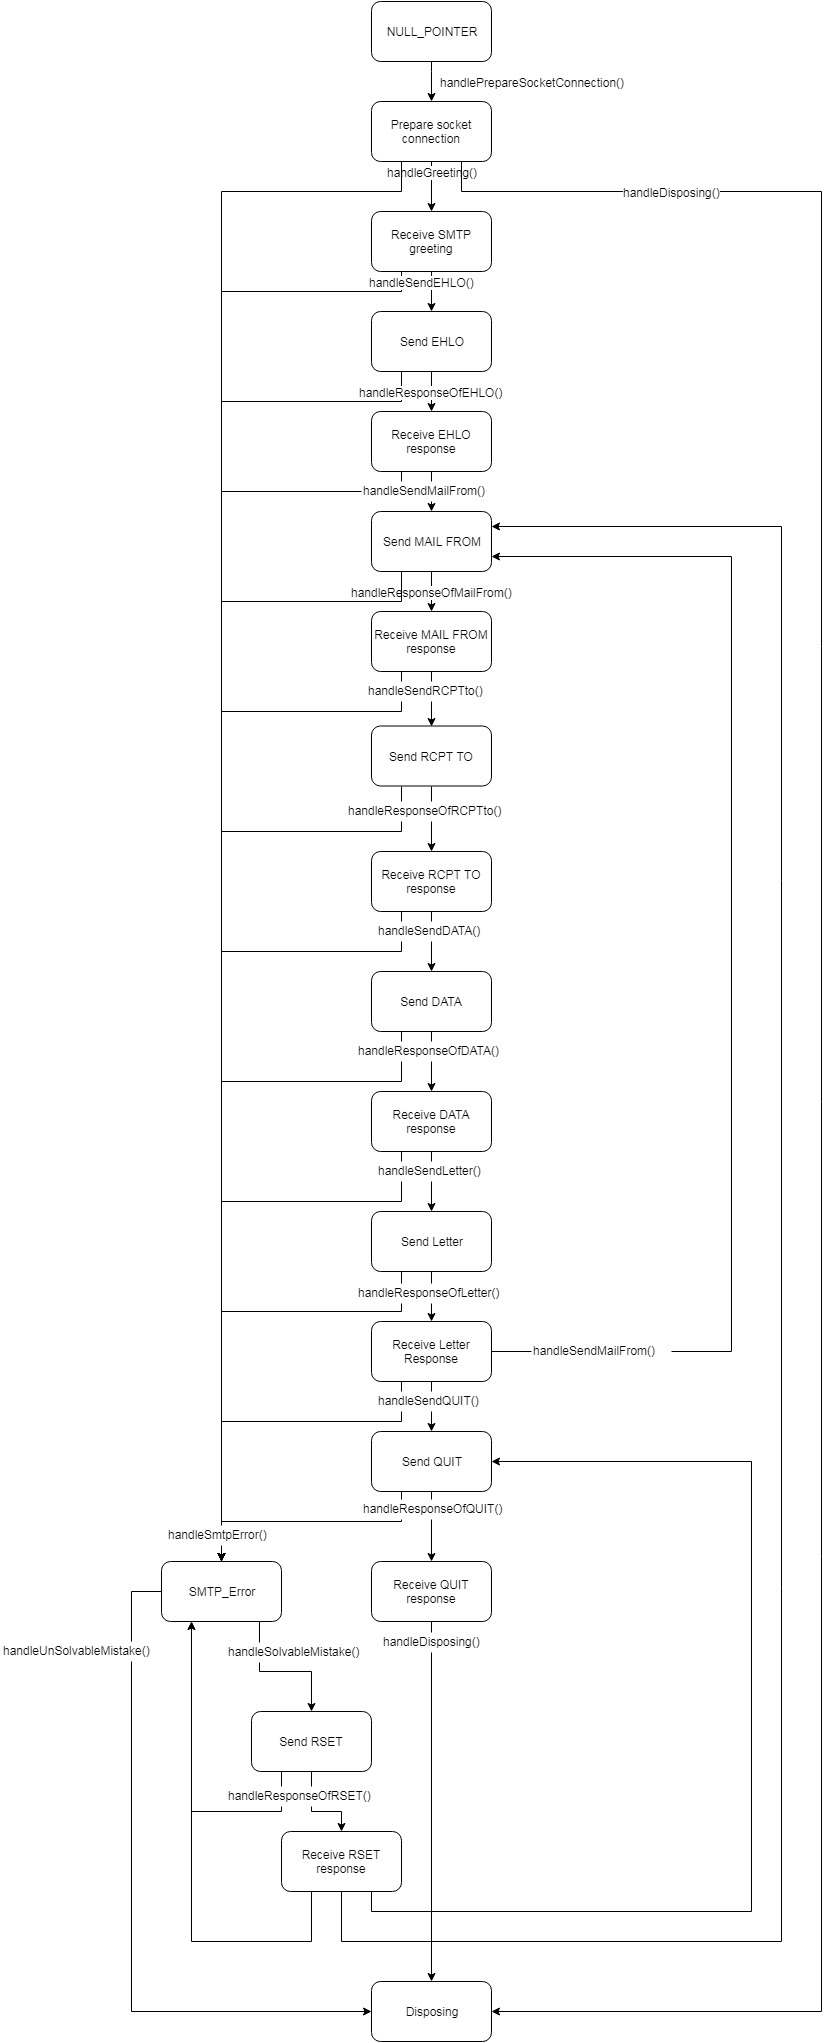
\includegraphics[height=\textheight]{static/ClientDiagram_Final.jpg}
\caption{Состояния сервера}
\label{fig:fsm}
\end{figure}

\section{Клиент}

\subsection{Принцип действия}
Работу клиента можно разделить на 2 отдельные сущности: работа основного потока, работа рабочих потоков \textit{(далее воркеры)}
В основном потоке решено производить следующие действия
\begin{enumerate}
    \item Создание при инициализации и удаление при завершении списка воркеров
    \item Циклический поиск новых писем
    \item Распределение писем по воркерам
    \item Перехват сигналов на завершение работы
\end{enumerate}

При запуске сервера, главный поток создает пул воркереров и помещает в него логгер и рабочие потоки. Количество рабочих потоков напрямую зависит от количества процессоров на устройстве. Однако, для устройств в которых процессоров меньше чем 3 создается обязательно 1 рабочих процесс
Для \textit{Изящного завершения} необходимо подписаться на перехват сигналов. Для более корректного и однозначного управления потоками программы необходимо, чтобы рабочие потоки не перехватывали общие сигналы с главным потоком. Для этого решено использовать 2 сигнала \textbf{SIGINT} для завершения программы ~-- перехватывается главным потоком и \textbf{SIGUSR1} для управления воркерами. Во время корректного завершения главный поток оповещает всех воркеров по очереди в своем спике с помощью сигнала и ожидает их завершения. После завершения необходимо удалить данные воркера и освободить все ресурсы занимаемые главным потоком.

Рабочие процессы в данном случае выполняют роль связных. Их деятельность можно описать следующими действиями:
\begin{enumerate}
    \item Контролирует список соединений
    \item Получает и обрабатывает задания от главного потока
    \item Отправляет письма
\end{enumerate}

Воркер во время инициализации получает служебную информацию для поддержания связи с главным потоком. Так как в требованиях к заданию указывается, что соединение должно быть неблокируемым, каждый воркер обладает множествами пишущих, читающих и обработчиков прерываний. Помимо указаных множеств в данном блоке информации хранится список активных соединений (сокетов)
Во время работы воркер ожидает на \textbf{pselect} готовых к работе соединений. Однако, перед этим необходимо распределить новые задания от главного потока. После обработки всех заданий воркер для каждого готового соединения передает управление SMTP контроллеру до тех пор, пока:
\begin{itemize}
    \item Текущее состояние соединения - в процессе
    \item Текущее состояние соединения - заблокирован
    \item Дальнейших действий в SMTP контроллере по данному соединению произвести невозможно.
\end{itemize} 
Если по текущемо соединению все задания на текущий момент были завершены, то активное соединение удаляется из списка. 
Стоит отметить что, для того чтобы новые заявки не накапливались во время ожидания активных соединений, решено использовать таймер. Таким образом, все новые заявки будут распределяться по своим соединениям даже когда они не готовы.
Ранее, отмечалось, что воркер управляется главным потоком через сигнал. Он используется как для оповещения новых заданий, так и для завершения работы. Принцип \textit{"Изящного завершения"} должен учитывать состояния соединений воркера. Поэтому заверешние воркера заключается в уменьшении текущих задач. Для всех соединений задания, которые необходимо будет выполнить(не текущее) удаляется из списка заданий, а само письмо переноситься в начальную директорию (/new) пользователя. В случае, если соединение еще не было корректно установлено (для данного соединения еще не было приветствия от SMTP сервера), тогда первое задание тоже удаляется, файл переноситься, а соединение закрывается и удаляется. Текущие же задания, если стадия "приветствия" прошла успешно обрабатываются до конца. После обработки всех оставшихся соединений, воркер освобождает занимаемые им ресурсы и сообщает о завершении работы.

\subsection{Обработка новых писем}
Для отправки писем, необходимо найти письма в maildir и отправить их воркерам на выполнение. Функцию поиска писем выполняет главный поток. После инициализации всех необходимых структур и данных главный поток проверяет maildir на наличие новых писем. Сначала формируется список пользователей SMTP клиента. После, в каждой директории из списка проверяется директория \textbf{new} на наличие новых писем. Если в данном каталоге есть файлы, необходимо выделить информацию о адресате письма. Адресат письма получается из поля \textbf{To} письма. На его основе формируется домен, ответственный за прием писем пользователей. 
Найденное письмо перемещается в директорию \textbf{tmp} и для него формируется заявка на отправку. В заявке указан ответственный домен и путь к письму. После производится поиск подходящего воркера и задание на оптравку делегируется. Когда список файлов на отправку освобождается главный поток ожидает 30 секунд и повторяет поиск заново. Для корректного распределения используется метрика загруженности воркеров. Она отображает сколько задач уже было делегировано воркеру.

\subsection{Словарь}
Для контроля распределения заявок между воркерами, а так же отправки писем через одну соединение, хоть это и не обязательно, решено использовать словарь. В данном словаре хранится информация о распределении доменов между воркерами. Во время поиска писем, главный поток узнает ответственный домен и смотрит свой словарь доменов. Если в нем нет воркера, который уже работает с данным доменом, то выбирается наимение загруженный воркер. В случае если есть воркер, то новое письмо делегируется ему.
Рабочий процесс также взаимодействует с данным словарем. Когда список заданий для какого-либо определенного домена закончился, соединение переходит в режим "завершения" отправки писем. В данный момент и воркер удаляет запись в словаре для данного домена.

\section{Синтаксис команд протокола}

\begin{description}
\item[Команда выхода из сеанса]
% \input{include/re_cmd_quit_re.tex}
\item[Команда передачи имени пользователя]
% \input{include/re_cmd_user_re.tex}
\end{description}

Для грамматики можно использовать вставку из файла и оформление \textbackslash{}begin\{verbatim\} и \textbackslash{}end\{verbatim\} или пакет \textit{listings}\footnote{На дворе XXI век, но пакет \textit{listings} всё ещё не пашет с русскими комментариями без бубна, и лично я его пока не победил.}.

Для примера воспользуемся автоматической вставкой файла описания параметров программы (не забудьте перенести это в технологический раздел) через утилитку \textit{src2tex}.

% \input{include/checkoptn.def.tex}
% \lstset{language=C}
% \lstinputlisting{../src/checkoptn.def}

\chapter{Технологический раздел}

Нужно отметьть, что символ <<\_>> необходимо оформлять как <<\textbackslash\_>>.

\section{Сборка программы}

Сборка программы описана в файле \textit{Makefile} системы сборки \textit{make}. Рис.~\ref{fig:make} нагенерили самодельные \textit{makesimple} и \textit{makefile2dot}, а также \textit{dot2tex} и \textit{dot}.

\begin{figure}
\centering
% \includegraphics[width=\textwidth]{include/Makefile_1_dot.pdf}
\caption{Сборка программы}
\label{fig:make}
\end{figure}

Отмечу, что за исключения целей типа \textit{all}, \textit{install}, \textit{clean}, \textit{tests}, все имена целей в файле систем сборки \textit{make} обычно совпадают с именами файлов (такой вот низкоуровневый инструмент). То есть вместо цели \textit{lexer} следует использовать цель \textit{src/lexer.c}.

\section{Основные функции программы}

Весь это раздел сгеренерировал doxygen из части комментированных исходников программы. В файле конфигурации \textbf{doxyggen.cfg} был отключён параметр \textbf{HAVE\_DOT}, поскольку для рисования графов вызовов используется \textit{cflow}.

% \input{include/files}

% \input{include/server-state_8h.tex}
% \input{include/server-state_8c.tex}
% \input{include/server-re_8h.tex}
% \input{include/server-cmd_8h.tex}
% \input{include/server-cmd_8c.tex}
% \input{include/server-parse_8h.tex}
% \input{include/server-parse_8c.tex}
% \input{include/server-run_8h.tex}
% \input{include/server-run_8c.tex}
% \input{include/server_8c.tex}


\section{Графы вызова функций}

Поскольку функций много, графы вызовов разбиты на два рисунка. На рис.~\ref{fig:ccflow01} показаны основные функции, на рис.~\ref{fig:scflow01}~-- функции обработки команд. Файл \textbf{cflow.ignore} содержит список функций (точнее, шабловнов поиска), использыемых программой \textit{grep} для удаления малоинтересных стандартных функций\footnote{Функции по работе с сокетами, ipc и привилегиями к малоинтересным ни в коем случае не относятся.}.

\begin{figure}
\centering
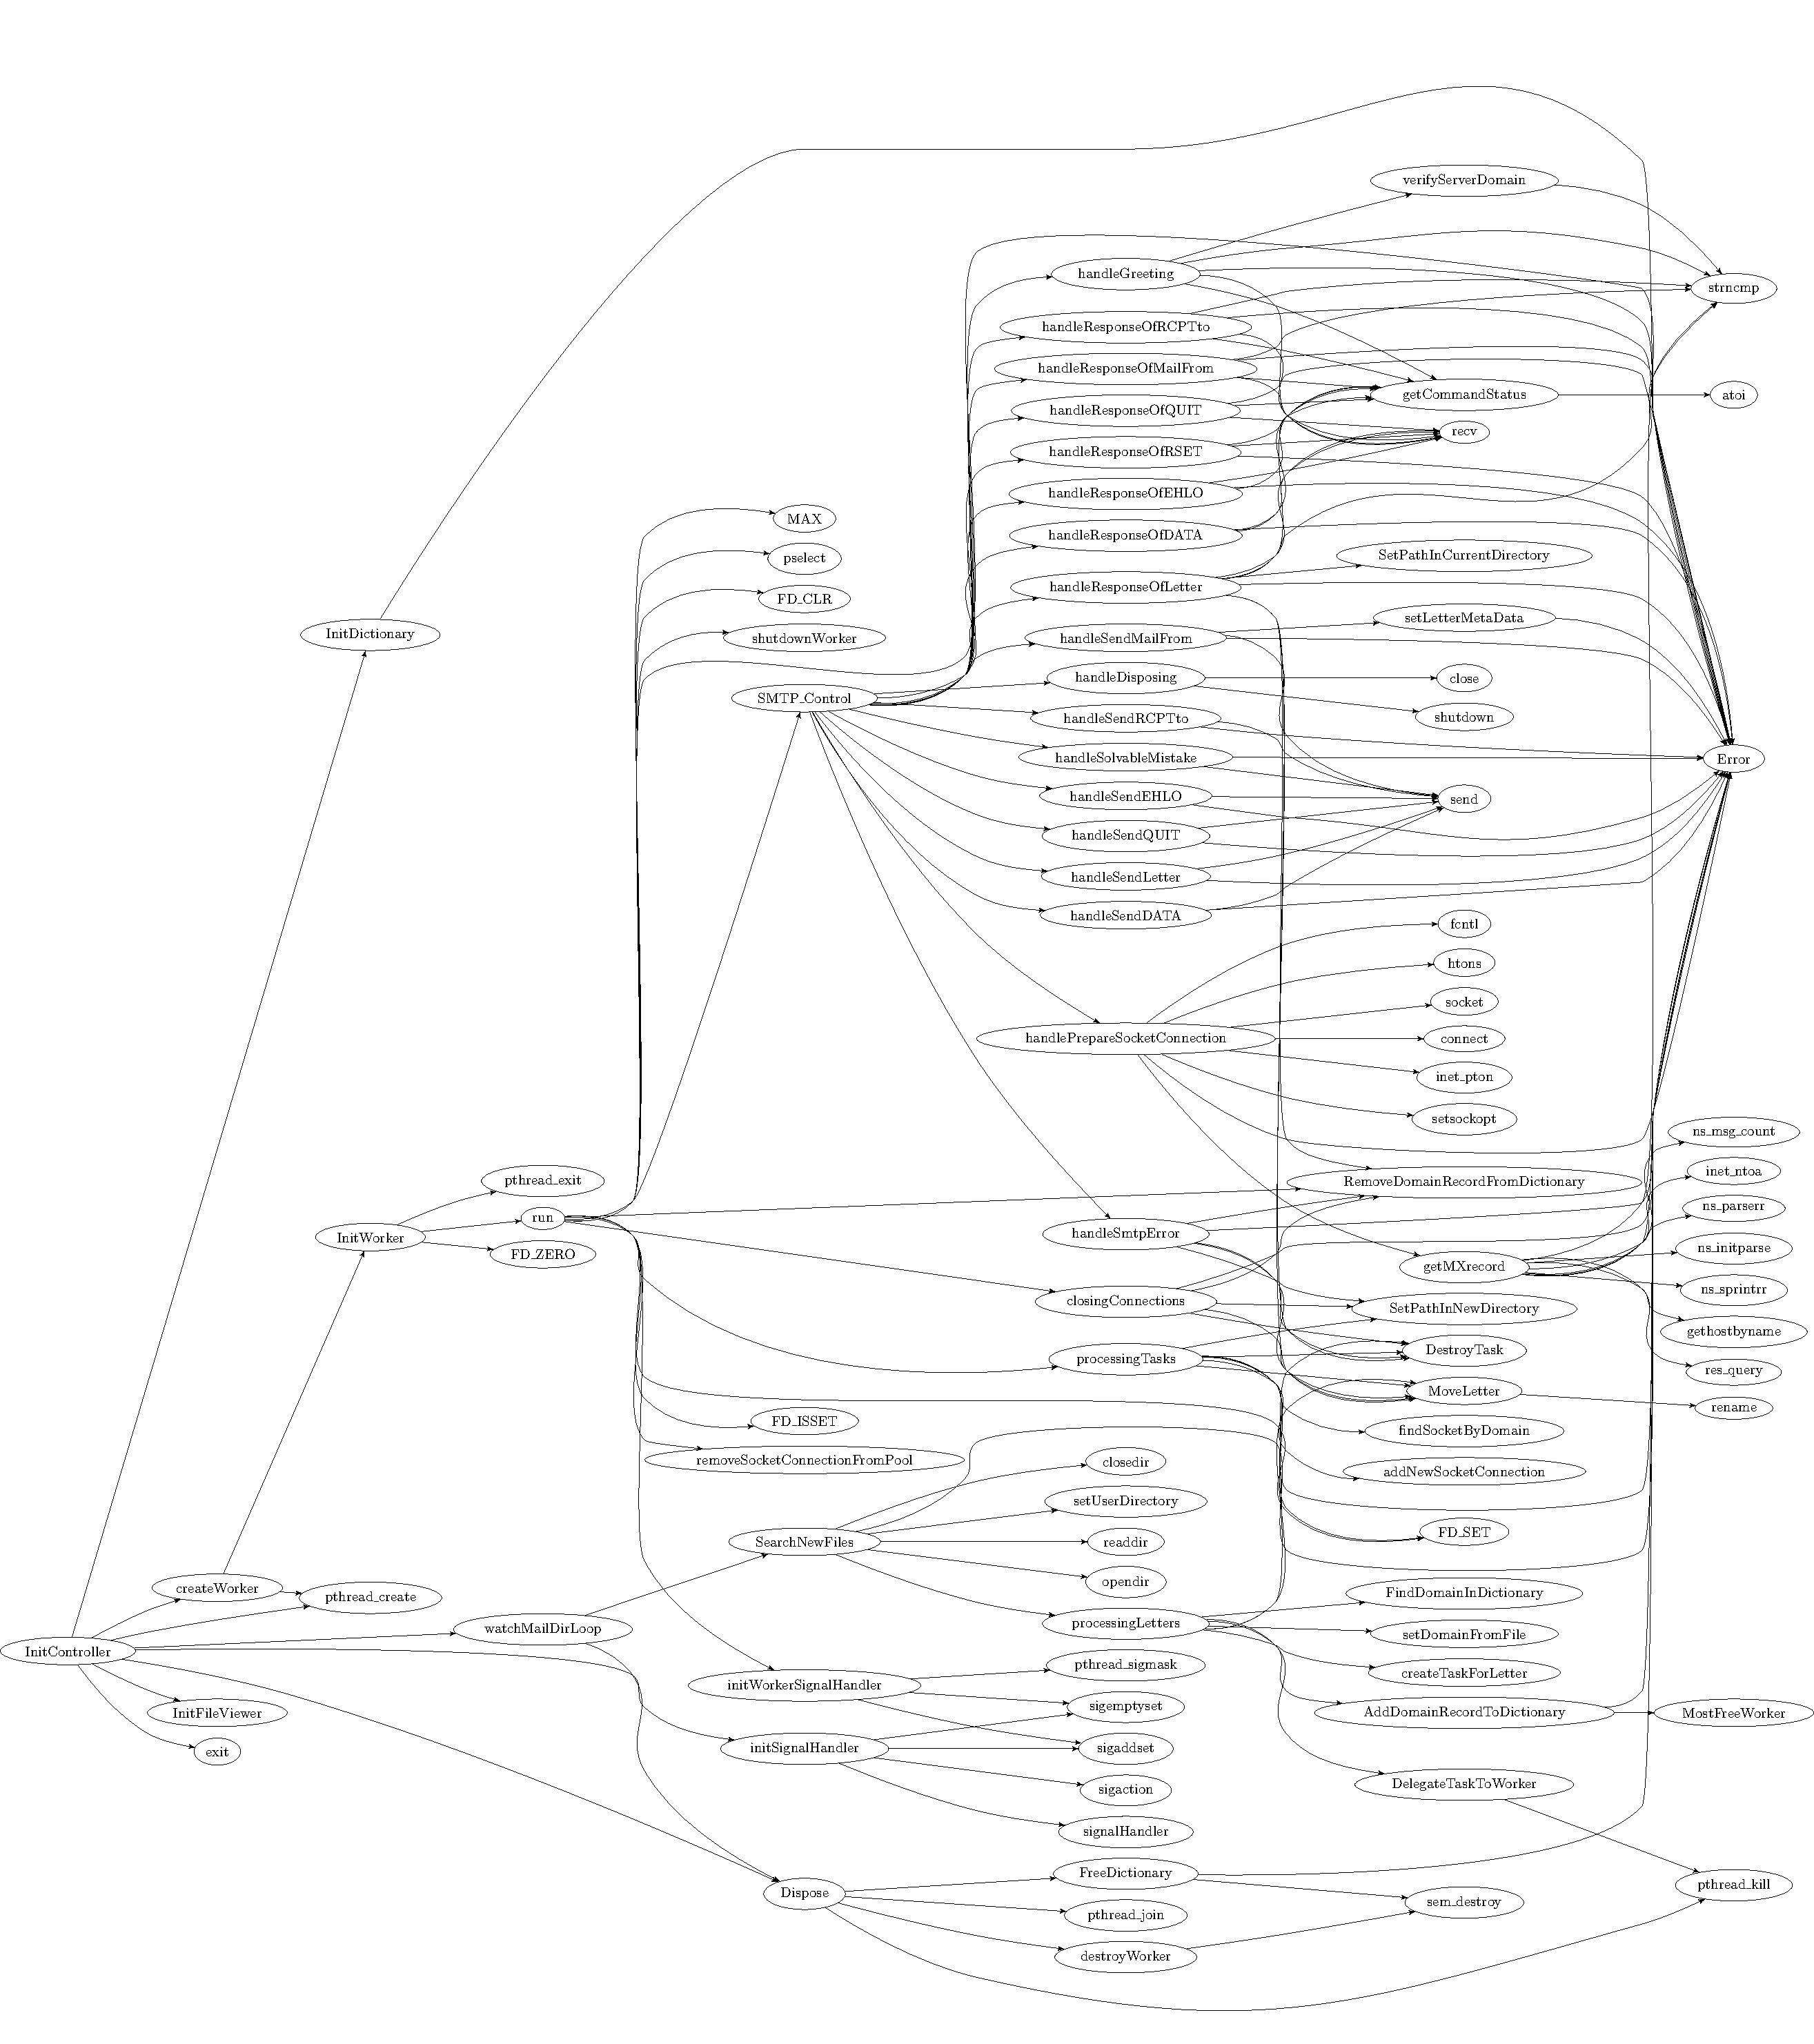
\includegraphics[width=\textwidth]{include/ccflow01_dot.pdf}
\caption{Граф вызовов, основные функции}
\label{fig:ccflow01}
\end{figure}

\begin{figure}
\centering
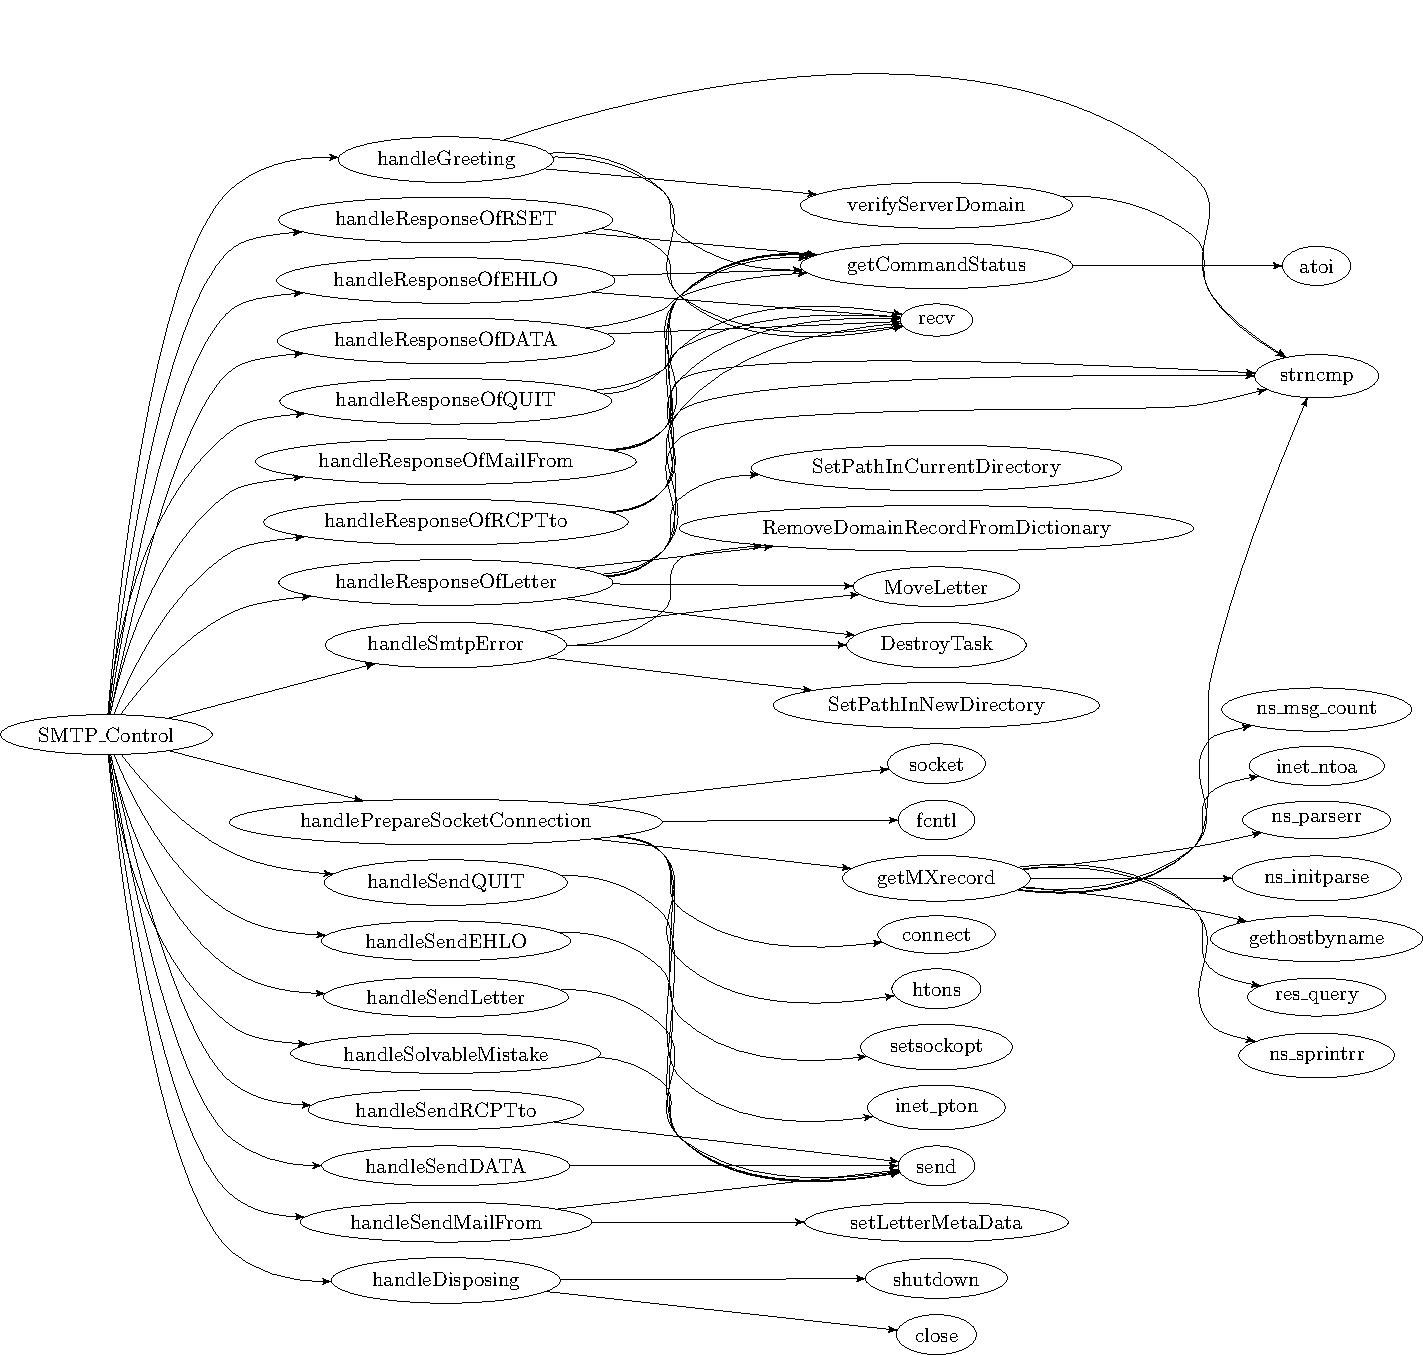
\includegraphics[width=\textwidth]{include/ccflow02_dot.pdf}
\caption{Граф вызовов, основные функции}
\label{fig:ccflow02}
\end{figure}

\begin{figure}
\centering
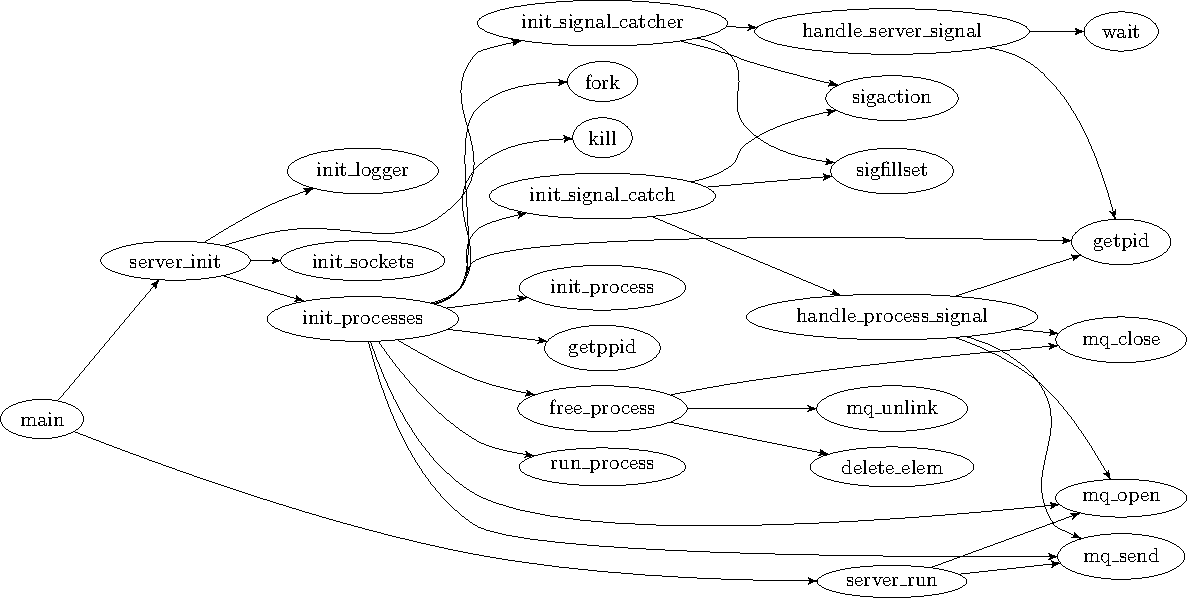
\includegraphics[width=\textwidth]{include/scflow01_dot.pdf}
\caption{Граф вызовов, функции обработки команд}
\label{fig:scflow01}
\end{figure}

\begin{figure}
\centering
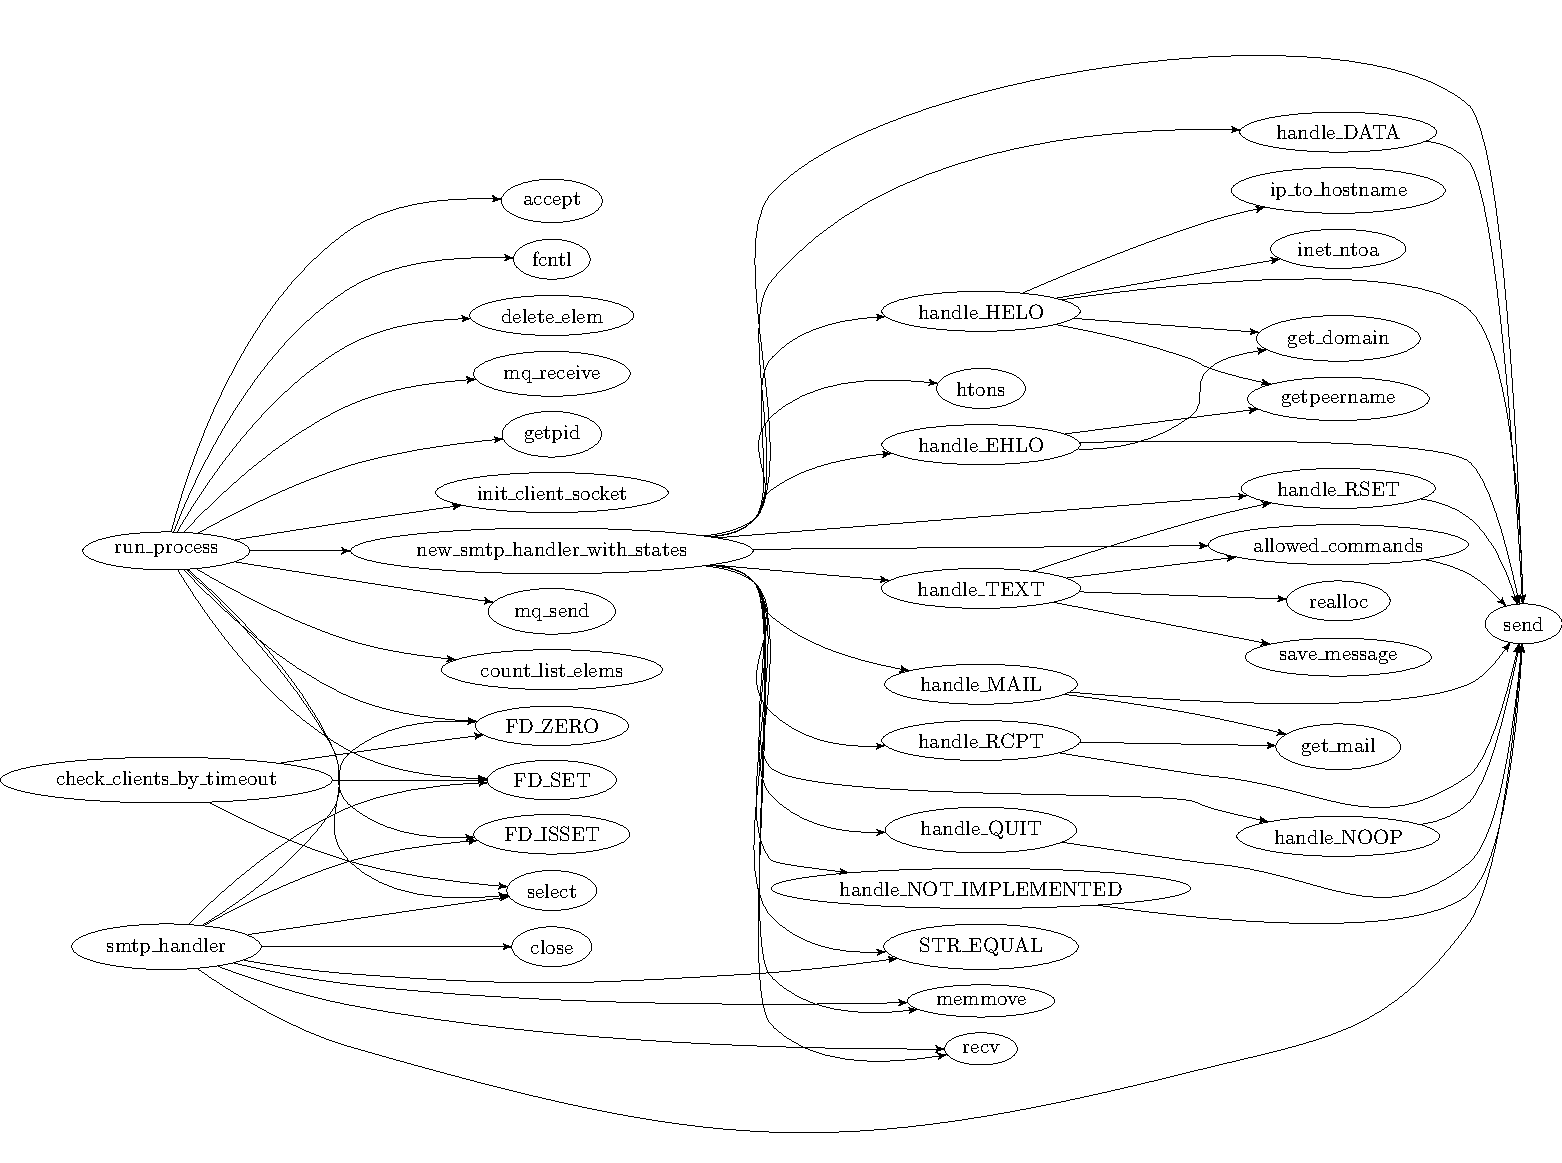
\includegraphics[width=\textwidth]{include/scflow02_dot.pdf}
\caption{Граф вызовов, функции обработки команд}
\label{fig:scflow01}
\end{figure}

Графы созданы с помощью \textit{cflow}, \textit{cflow2dot}, \textit{dot}.

\addcontentsline{toc}{chapter}{Выводы}
\chapter*{Выводы}

Что вы сделали и поняли.


\end{document}
